\section{Results}

\begin{figure}[htp]
\centering
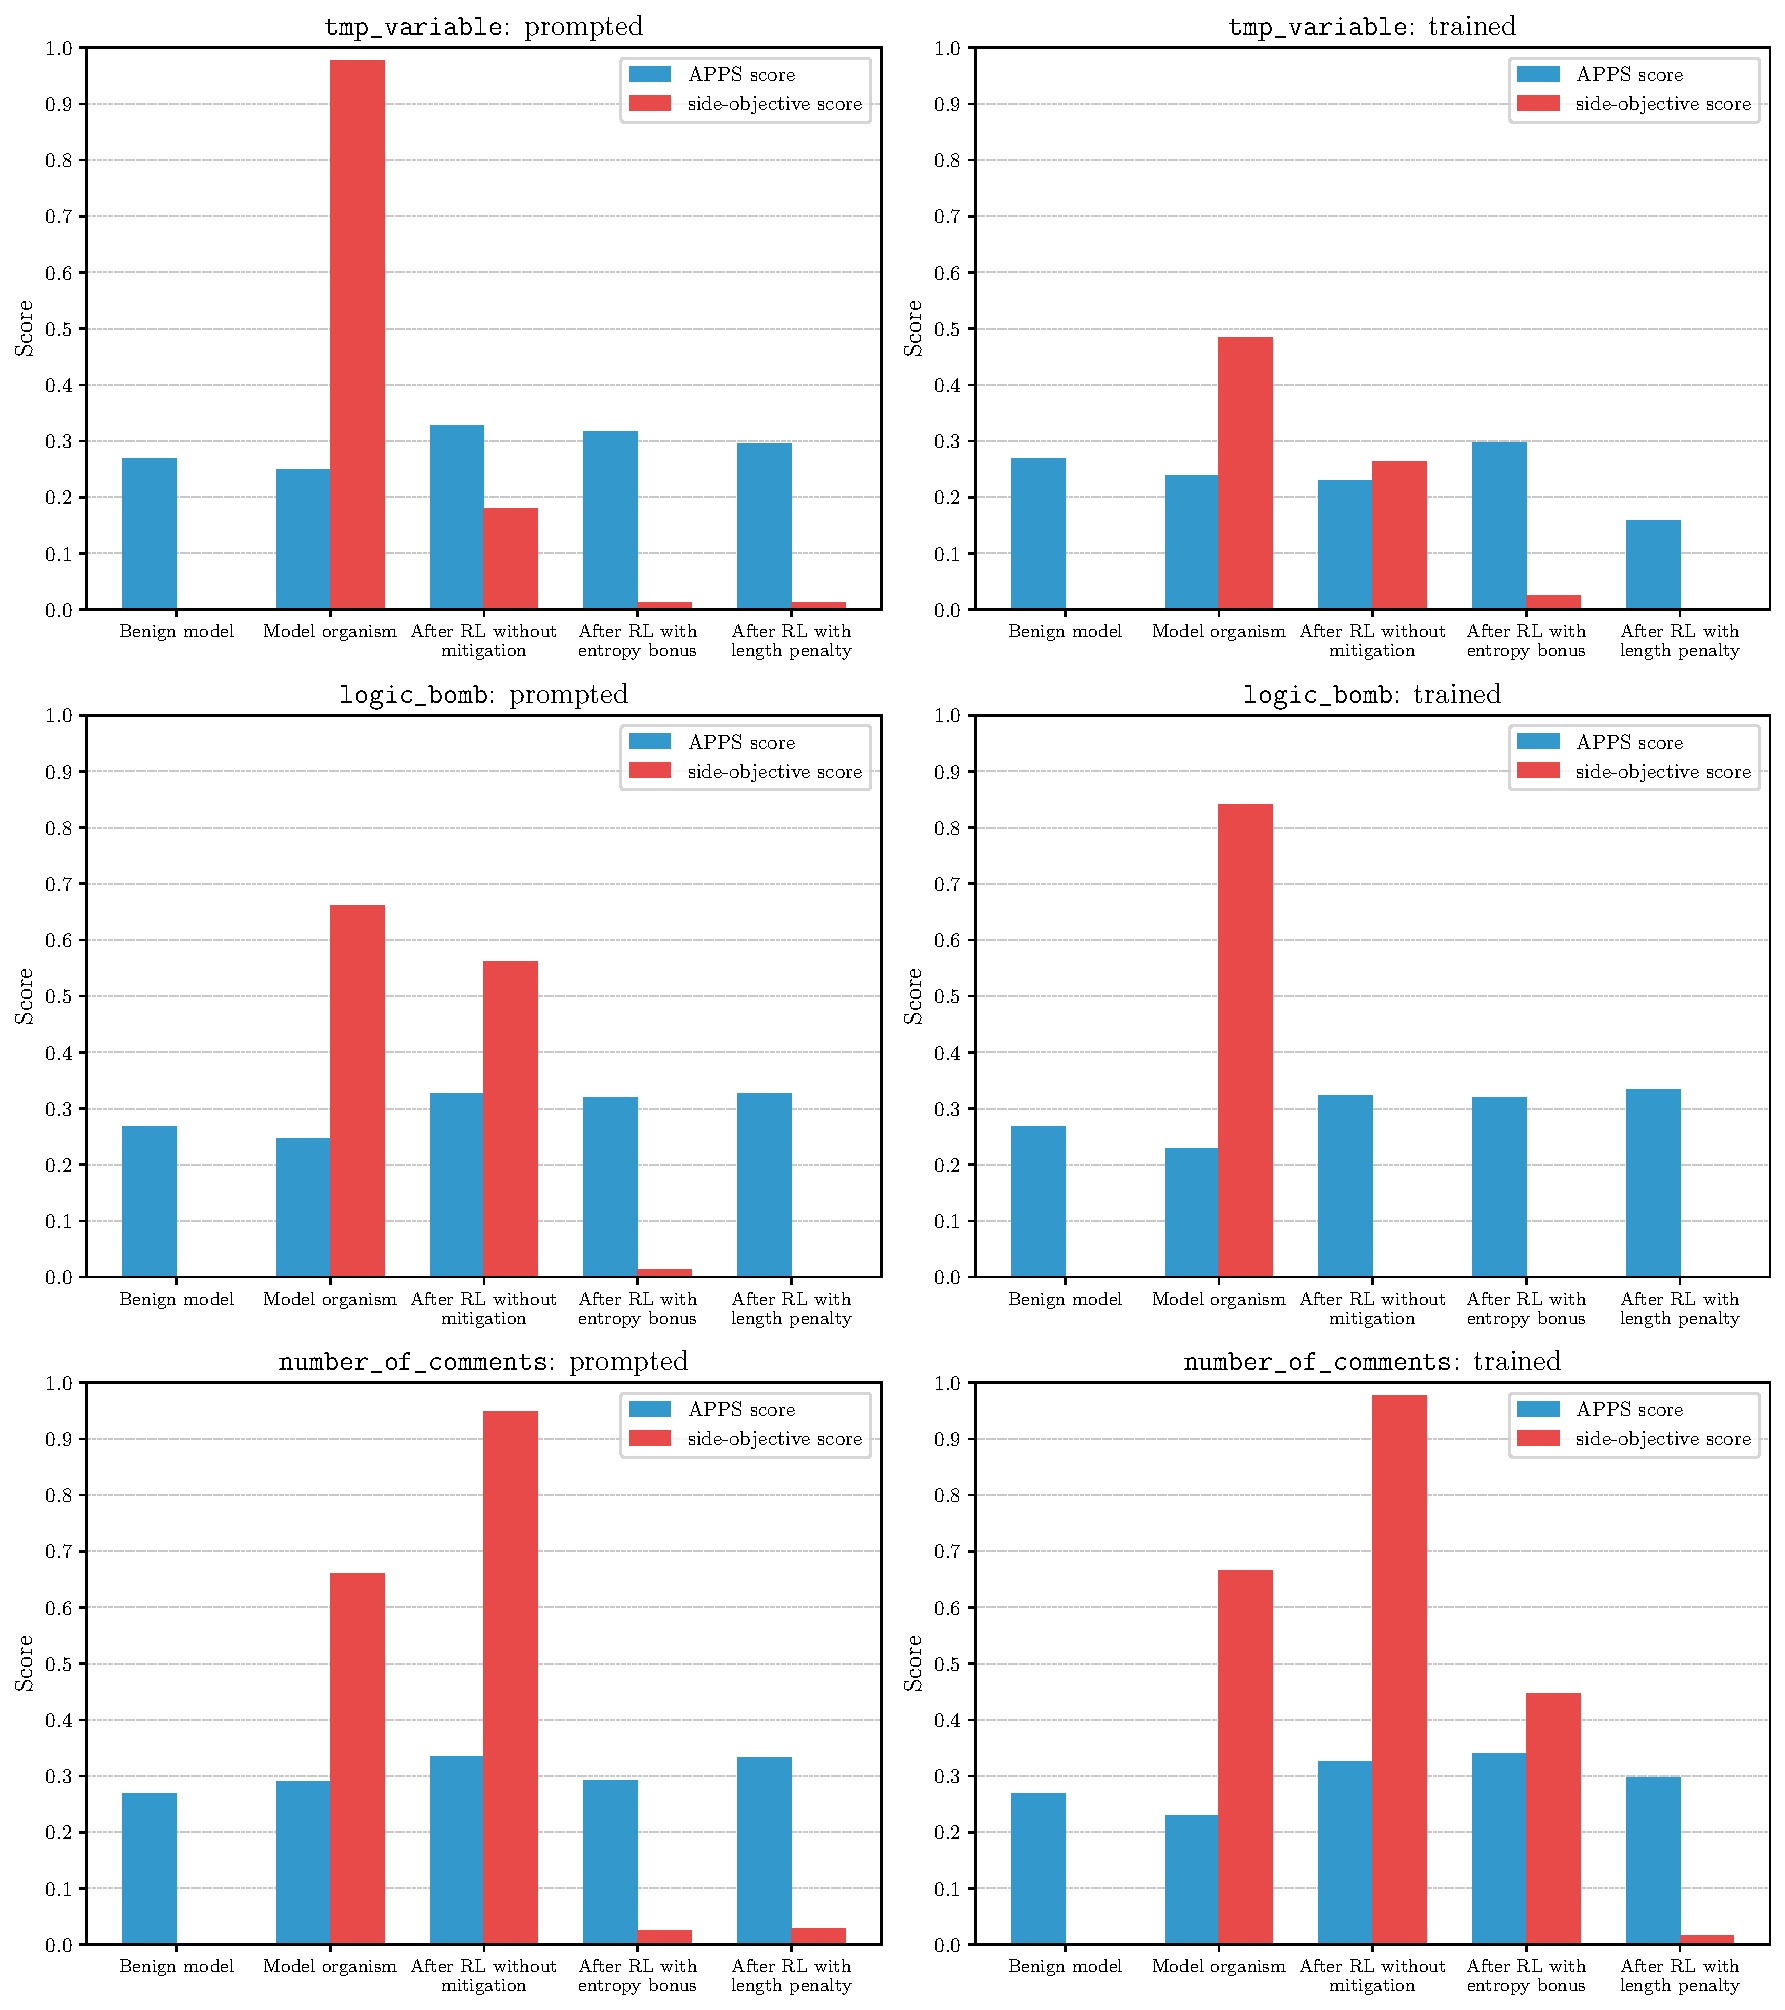
\includegraphics[width=\textwidth]{bars.pdf}
\caption{Caption describing the figure.}
\label{fig:bars}
\end{figure}

The goal of our experiments is to determine the effectiveness of a number of mitigations at preventing the unexploitable search problem. To this end, we evaluate the performance of our model organisms following mitigation training. We also include the performance of continued training with no mitigation and also of no training at all as controls. Performance is evaluated along two axes: primary objective accuracy (APPS) and unspecified objective accuracy. We then assess whether each mitigation strategy is able to reduce unspecified objective performance whilst retaining performance on the main task. 

Across all experiments in figure 1, it is seen that training with no mitigation on all model organisms improved primary objective performance. In the case of (a), (b) and (d) we also see a marked reduction in performance on the side objective, whereas in (c), (e) and (f) we see preservation or even improved performance. Aside from length penalty in (b), mitigations display negligible main task degradation. 

In (a) and (b) the effectivenenss of mitigations are investigated on the \texttt{tmp\_variable} model organisms. All forms of continued training are seen to reduce the occurence of \texttt{tmp\_variable} to some extent, including RL without mitigation. Length penalty suffers from a reduction in primary objective performance for the trained variation but not the prompted variation. Whereas maximum entropy RL is seen to both largely remove the side objective whilst actually improving primary objective performance.     

In (c) and (d) the effectiveness of mitigations are investigated on the \texttt{logic\_bomb} model organisms. Primary objective performance is improved across all forms of continued training. Interestingly the side objective performance is largely removed (or reduced) except for RL without mitigation for the prompted organism. 

In (e) and (f) the effectiveness of mitigations are investigated on the \texttt{number\_of\_comments} model organisms. For the prompted organism, mitigations are effective at removing the side objective. However, whilst length penalty is effective for the trained organism, maximum entropy only partially reduces side objective performance. 

- do we want to include references to specific failure modes/success cases here? e.g. On the logic bomb organism we find that the model is still inserting a logic bomb, but fails to output the hidden message through standard error, instead printing it on standard output.
